
\section{some side channel examples}

\subsection{example: check\_passphrase}

\begin{frame}[fragile]{check\_passphrase}
\begin{lstlisting}[style=smaller,language=C]
int check_passphrase(const char *versus) {
    int i = 0;
    while (passphrase[i] == versus[i] &&
           passphrase[i]) {
        i += 1;
    }
    return (passphrase[i] == versus[i]);
}
\end{lstlisting}
\begin{itemize}
\item<2> number of iterations = number matching characters
\item<2> leaks information about passphrase, oops!
\end{itemize}
\end{frame}

\begin{frame}{exploiting check\_passphrase (1)}
\begin{tabular}{ll}
guess & measured time \\ \hline
aaaa & $100\pm5$ \\
baaa & $103\pm4$ \\
caaa & $102\pm6$ \\
\myemph{daaa} & \myemph{$111\pm5$} \\
eaaa & $99 \pm6$ \\
faaa & $101\pm7$ \\
gaaa & $104\pm4$ \\
\ldots & \ldots \\
\end{tabular}
\end{frame}

\begin{frame}{exploiting check\_passphrase (2)}
\begin{tabular}{ll}
guess & measured time \\ \hline
daaa & $102\pm5$ \\
dbaa & $ 99\pm4$ \\
dcaa & $104\pm4$ \\
ddaa & $100\pm6$ \\
deaa & $102\pm4$ \\
\myemph{dfaa} & \myemph{$109\pm7$} \\
dgaa & $103\pm4$ \\
\ldots & \ldots \\
\end{tabular}
\end{frame}



\subsection{timing and ciphers}

\begin{frame}{timing and cryptography}
    \begin{itemize}
    \item lots of asymmetric cryptography uses big-integer math
    \item example: multiplying 500+ bit numbers together
    \vspace{.5cm}
    \item how do you implement that?
    \end{itemize}
\end{frame}

\begin{frame}{big integer multiplcation}
    \begin{itemize}
    \item say we have two 64-bit integers $x$, $y$
        \begin{itemize}
        \item and want to 128-bit product, but our multiply instruction only does 64-bit products
        \end{itemize}
    \item one way to multiply:
    \vspace{.5cm}
    \item divide $x$, $y$ into 32-bit parts: $x=x_1\cdot2^{32}+x_0$ and $y=y_1\cdot2^{32}+y_0$
    \item then $xy = x_1y_12^{64}+x_1y_0\cdot2^{32}+x_0y_1\cdot2^{32}+x_0y_0$
    \vspace{.5cm}
    \item<2-> can extend this idea to arbitrarily large numbers
    \item<2-> \myemph{number of smaller multiplies depends on size of numbers!}
    \end{itemize}
\end{frame}

\begin{frame}{big integers and cryptography}
    \begin{itemize}
    \item naive multiplication idea:
        \begin{itemize}
        \item number of steps depends on size of numbers
        \end{itemize}
    \item problem: sometimes the value of the number is a secret
        \begin{itemize}
        \item e.g. part of the private key
        \end{itemize}
    \item oops! revealed through timing
    \end{itemize}
\end{frame}

\begin{frame}{big integer timing attacks in practice (1)}
    \begin{itemize}
    \item early versions of OpenSSL (TLS implementation)had timing attack
        \begin{itemize}
        \item Brumley and Boneh, ``Remote Timing Attacks are Practical'' (Usenix Security '03)
        \end{itemize}
    \item attacker could figure out bits of private key from timing
    \vspace{.5cm}
    \item why? variable-time mulitplication and modulus operations 
        \begin{itemize}
        \item got faster/slower depending on how input was related to private key
        \end{itemize}
    \end{itemize}
\end{frame}

\begin{frame}{big integer timing attacks in practice (2)}
    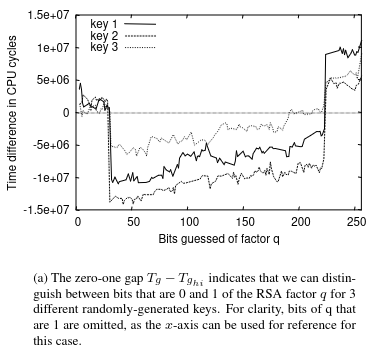
\includegraphics[height=0.9\textheight]{../spectre/remote-timing-prac-fig3a}
    \imagecredit{Figure 3a from Brumley and Boneh, ``Remote Timing Attacks are Practical''}
\end{frame}


\subsection{example: which website}

\begin{frame}{browsers and website leakage}
    \begin{itemize}
    \item web browsers run code from untrusted webpages
    \item one goal: can't tell what other webpages you visit
    \end{itemize}
\end{frame}

\begin{frame}[fragile]{some webpage leakage (1)}
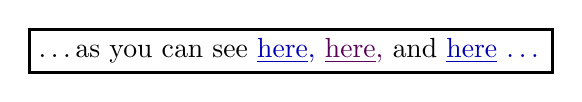
\begin{tikzpicture}
\node[draw,very thick] {
    \ldots as you can see \color{blue!70!black}{\underline{here}}, \color{violet!70!black}{\underline{here}},
    \color{black!70!black}{and} \color{blue!70!black}{\underline{here}} \ldots
};
\end{tikzpicture}
\begin{itemize}
\item convenient feature 1: browser marks visited links
\end{itemize}
\begin{tikzpicture}
\node[draw,very thick,align=left] {
\begin{lstlisting}[style=smaller,language={}]
<script>
var the_color = window.getComputedStyle(
    document.querySelector('a[href=~"foo.com"]')
).color
if (the_color == ...) { ... }
</script>
\end{lstlisting}
};
\end{tikzpicture}
\begin{itemize}
\item \sout<2->{convenient feature 2: scripts can query current color of something}
    \begin{itemize}
    \item<2-> fix 1: getComputedStyle lies about the color
    \item<2-> fix 2: limited styling options for visited links
    \end{itemize}
\end{itemize}
\end{frame}

\begin{frame}{some webpage leakage (2)}
\begin{itemize}
\item one idea: script in webpage times loop that writes big array
\item variation in timing depends on \myemph{other things running on machine}
\end{itemize}
\begin{tikzpicture}
\begin{visibleenv}<2->
\node (pic) {
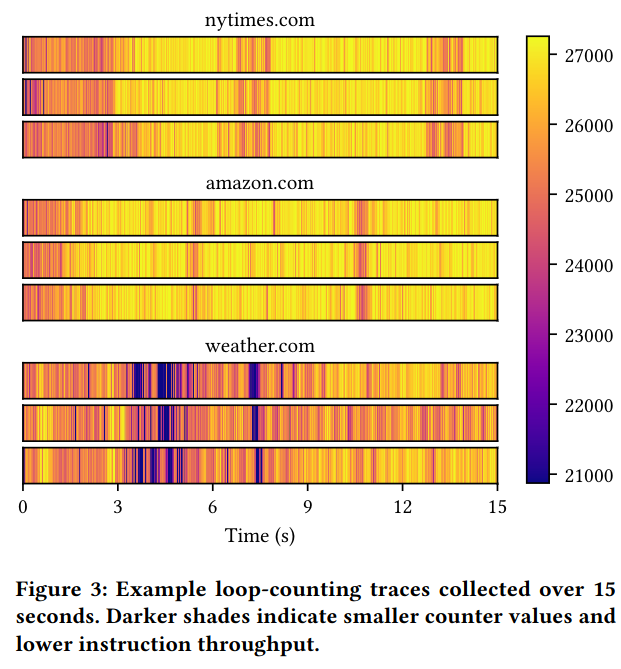
\includegraphics[height=0.6\textheight]{../spectre/website-sigs-fig}
};
\node[anchor=north west,align=left] at (pic.north east) {
turns out, other webpages \\
create distinct ``signatures'' \\
\fontsize{8}{9}\selectfont\parbox{10cm}{Figure from Cook et al, ``There’s Always a Bigger Fish:
Clarifying Analysis of a Machine-Learning-Assisted Side-Channel Attack'' (ISCA '22)}
};
\end{visibleenv}
\end{tikzpicture}
\end{frame}


% FIXME: \subsection{example: RF leaks}

% FIXME: \subsection{example: power analysis}

% FIXME: based on https://search.iczhiku.com/paper/U27SsPw1R1KrhDKc.pdf % Crypto'99 DPA paper

\section{cache side channels}

\subsection{introduction: observing cache evictions}

\begin{frame}{inferring cache accesses (1)}
\begin{itemize}
\item suppose I time accesses to array of chars:
    \begin{itemize}
    \item reading array[0]: 3 cycles
    \item reading array[64]: 4 cycles
    \item reading array[128]: 4 cycles
    \item reading array[192]: 20 cycles
    \item reading array[256]: 4 cycles
    \item reading array[288]: 4 cycles
    \item \ldots
    \end{itemize}
\item what could cause this difference?
    \begin{itemize}
    \item array[192] not in some cache, but others were
    \end{itemize}
\end{itemize}
\end{frame}

\begin{frame}[fragile,label=cacheAccess]{inferring cache accesses (2)}
some psuedocode:
\begin{lstlisting}[language=C,style=smaller]
char array[CACHE_SIZE];
AccessAllOf(array);
*other_address += 1;
TimeAccessingArray();
\end{lstlisting}
\begin{itemize}
\item suppose during these accesses I discover that
    \texttt{array[128]} is slower to access
\item probably because \texttt{*other\_address} loaded into cache + evicted it
\item what do we know about \texttt{other\_address}? (select all that apply)
\end{itemize}
\small
\begin{tabular}{lll}
A. same cache tag & B. same cache index & C. same cache offset \\
D. diff. cache tag & E. diff. cache index & F. diff. cache offset \\
\end{tabular}
\end{frame}


\begin{frame}{some complications}
    \begin{itemize}
    \item caches often use physical, not virtual addresses
        \begin{itemize}
        \item (and need to know about physical address to compare index bits)
        \item (but can infer physical addresses with measurements/asking OS)
        \item (often OS allocates contiguous physical addresses esp. w/`large pages')
        \end{itemize}
    \item storing/processing timings evicts things in the cache
        \begin{itemize}
        \item (but can compare timing with/without access of interest to check this)
        \end{itemize}
    \item processor ``pre-fetching'' may load things into cache before access is timed
        \begin{itemize}
            \item (but can arrange accesses to avoid triggering prefetcher \\
                and make sure to measure with memory barriers)
        \end{itemize}
    \item some L3 caches use a simple hash function to select index instead of  index bits
    \end{itemize}
\end{frame}


    % FIXME:
        % setup example 1:
            % fill cache; do something that accesses var part; time accessing everything --- slower if ___

\subsection{exercise: detect this access? (DM)}
\begin{frame}[fragile]{exercise: inferring cache accesses (1)}
\begin{lstlisting}[language=C,style=smaller]
char *array;
array = AllocateAlignedPhysicalMemory(CACHE_SIZE);
LoadIntoCache(array, CACHE_SIZE);
if (mystery) {
    *pointer += 1;
}
if (TimeAccessTo(&array[index]) > THRESHOLD) {
    /* pointer accessed */
}
\end{lstlisting}
\begin{itemize}
    \item suppose \texttt{pointer} is \texttt{0x1000188}
\item and cache (of interest) is direct-mapped, 32768 ($2^{15}$) byte, 64-byte blocks
\item what array index should we check?
\end{itemize}
\end{frame}

\begin{frame}<0>[label=inferCache1Soln,fragile]{solution}
\begin{lstlisting}[language=C,style=script]
array = AllocateAlignedPhysicalMemory(CACHE_SIZE);
LoadIntoCache(array, CACHE_SIZE);
if (mystery) { *pointer = 1; }
if (TimeAccessTo(&array[index]) > THRESHOLD) { /* pointer accessed */ }
\end{lstlisting}
\begin{itemize}
    \item $2^{15}$ byte direct mapped cache, $64=2^{6}$ byte blocks
    \item \myemph<2>{9 index bits}, 6 offset bits
    \item \texttt{0x1000188}: \texttt{\ldots 0\myemph<2>{\textit{000 0001 10}}00 1000}
    \vspace{.5cm}
    \item \texttt{array[0]} starts at multiple of cache size --- index 0, offset 0
    \item to get index 6, offset 0 array[\texttt{0b\myemph{\textit{1 10}}00 0000}] = array[\texttt{0x180}]
\end{itemize}
\end{frame}

\iftoggle{heldback}{}{\againframe<1->{inferCache1Soln}}

\begin{frame}[label=inferCache1Aside,fragile]{aside}
\begin{lstlisting}[language=C,style=smaller]
array = AllocateAlignedPhysicalMemory(CACHE_SIZE);
LoadIntoCache(array, CACHE_SIZE);
if (mystery) { *pointer += 1; }
if (TimeAccessTo(&array[index]) > THRESHOLD) {
    /* pointer accessed */
}
\end{lstlisting}
\begin{itemize}
    \item will this detect when pointer accessed? yes
    \item will this detect if mystery is true? not quite
    \item \ldots because branch prediction could started cache access
\end{itemize}
\end{frame}


\begin{frame}[fragile]{exercise: inferring cache accesses (2)}
\begin{lstlisting}[language=C,style=smaller]
char *other_array = ...;
char *array;
array = AllocateAlignedPhysicalMemory(CACHE_SIZE);
LoadIntoCache(array, CACHE_SIZE);
other_array[mystery] += 1;
for (int i = 0; i < CACHE_SIZE; i += BLOCK_SIZE) {
    if (TimeAccessTo(&array[i]) > THRESHOLD) {
        /* found something interesting */
    }
}
\end{lstlisting}
\begin{itemize}
\item other\_array at 0x200400, and interesting index is i=0x800,
    then what was mystery?
\end{itemize}
\end{frame}

\begin{frame}<0>[label=inferCache2Soln,fragile]{solution}
\begin{lstlisting}[language=C,style=script]
array = AllocateAlignedPhysicalMemory(CACHE_SIZE);
LoadIntoCache(array, CACHE_SIZE);
other_array[mystery] += 1;
for (int i = 0; i < CACHE_SIZE; i += BLOCK_SIZE) {
    if (TimeAccessTo(&array[i]) > THRESHOLD) { ... }
}
\end{lstlisting}
\begin{itemize}
    \item at i=0x800: \texttt{\ldots 0\myemph{\textit{000 1000 00}}00 0000} (cache index = 0x20)
    \item other\_array at \texttt{0x200400}
    \item Q: \texttt{0x200400 + X} has cache index 0x20? 
\end{itemize}
{\tt\small
\begin{tabular}{l|lll}
0x200400 & \ldots 0 & \myemph{000 0100 00} & 00 0000 \\
+ X      & \ldots ? & \myemph{000 0100 00} & ?? ???? \\ \hline
    0x200400+X & \ldots ? & \myemph{000 1000 00} & ?? ???? \\
\end{tabular}
}
\end{frame}

\iftoggle{heldback}{}{\againframe<1->{inferCache2Soln}}

\subsection{exercise: detect this access? (2-way)}


\begin{frame}[fragile]{exercise: inferring cache accesses (2)}
\begin{lstlisting}[language=C,style=smaller]
char *array;
posix_memalign(&array, CACHE_SIZE, CACHE_SIZE);
LoadIntoCache(array, CACHE_SIZE);
if (mystery) {
    *pointer = 1;
}
if (TimeAccessTo(&array[index1]) > THRESHOLD ||
    TimeAccessTo(&array[index2]) > THRESHOLD) {
    /* pointer accessed */
}
\end{lstlisting}
\begin{itemize}
\item pointer is 0x1000188
\item cache is 2-way, 32768 ($2^{15}$) byte, 64-byte blocks, ???? replacement
\item what array indexes should we check?
\end{itemize}
\end{frame}


\subsection{PRIME+PROBE, AES example}
\begin{frame}{PRIME+PROBE}
    \begin{itemize}
    \item name in literature: PRIME + PROBE
    \item PRIME: fill cache (or part of it) with values
    \item do thing that uses cache
    \item PROBE: access those values again and see if it's slow
    \vspace{.5cm}
    \item (one of several ways to measure how cache is used)
    \vspace{.5cm}
    \item coined in attacks on AES encryption
    \end{itemize}
\end{frame}

\begin{frame}{example: AES (1)}
\begin{itemize}
\item from Osvik, Shamir, and Tromer, ``Cache Attacks and Countermeasures: the Case of AES'' (2004)
\item early AES implementation used lookup table
\item goal: detect index into lookup table
    \begin{itemize}
    \item index depended on key + data being encrypted
    \end{itemize}
\item tricks they did to make this work
    \begin{itemize}
    \item vary data being encrypted
    \item subtract average time to look for what changes
    \item lots of measurements
    \end{itemize}
\end{itemize}
\end{frame}

\begin{frame}{example: AES (2)}
\small from Osvik, Shamir, and Tromer, ``Cache Attacks and Countermeasures: the Case of AES'' (2004) \\
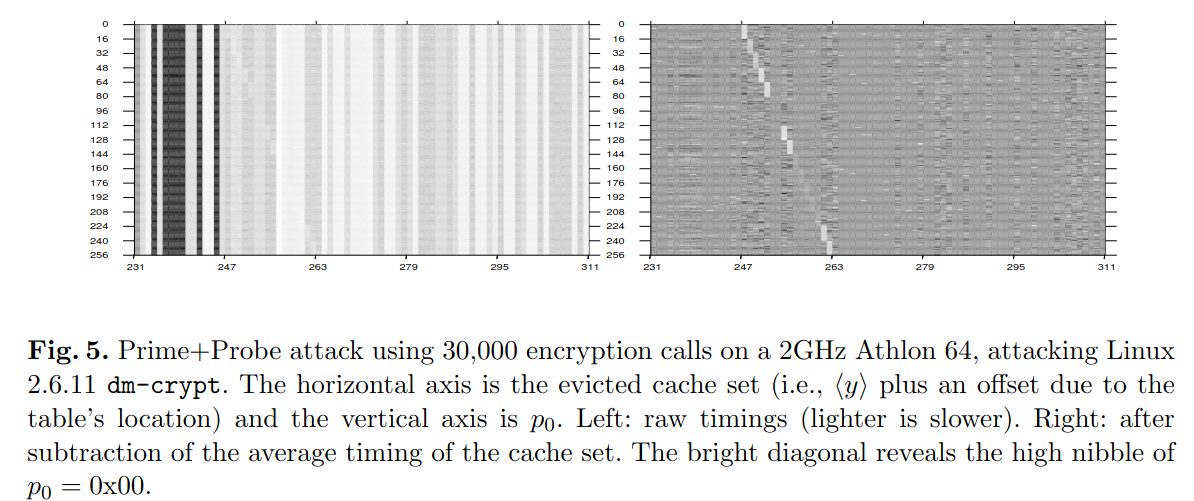
\includegraphics[width=1.0\textwidth]{../spectre/prime-probe-osvik}
\end{frame}
 % FIXME: lfence-using example

\subsection{reading a value (1)}
\begin{frame}[fragile]{reading a value}
\begin{lstlisting}[language=C,style=smaller]
char *array;
posix_memalign(&array, CACHE_SIZE, CACHE_SIZE);
AccessAllOf(array);
other_array[mystery * BLOCK_SIZE] += 1;
for (int i = 0; i < CACHE_SIZE; i += BLOCK_SIZE) {
    if (CheckIfSlowToAccess(&array[i])) {
        ...
    }
}
\end{lstlisting}
\begin{itemize}
\item with 32KB direct-mapped cache
\item suppose we find out that \texttt{array[0x400]} is slow to access
\item and other\_array starts at address 0x100000
\item what was mystery?
\end{itemize}
\end{frame}


\section{seeing speculation via side channels}

\subsection{revising array lookup}

\usetikzlibrary{matrix}
\begin{frame}[fragile]{revisiting an earlier example (1)}
\begin{lstlisting}[language=C,style=smaller]
char *array;
posix_memalign(&array, CACHE_SIZE, CACHE_SIZE);
LoadIntoCache(array, CACHE_SIZE);
if (mystery) {
    *pointer += 1;
}
if (TimeAccessTo(&array[index]) > THRESHOLD) {
    /* pointer accessed */
}
\end{lstlisting}
\begin{itemize}
\item what if mystery is false \textit{but} branch mispredicted?
\end{itemize}
\end{frame}

\begin{frame}[fragile]{revisiting an earlier example (2)}
\lstset{language=myasm}
\begin{tikzpicture}
\tikzset{
    forwardLine/.style={blue!60!black,thick,-Latex},
    hiForwardOn/.style={alt=#1{blue}{}},
    forwardLineB/.style={red,dashed,thick,-Latex},
    sepLine/.style={black!40,densely dotted},
};
\tikzset{
    fetch/.style={fill=red!15},
    decode/.style={fill=orange!15},
    rename/.style={fill=yellow!15},
    issue/.style={fill=yellow!15!green!15},
    execute/.style={fill=blue!15},
    memory/.style={fill=blue!15},
    writeback/.style={fill=violet!15},
    commit/.style={fill=magenta!20},
}
\newcommand{\fdemw}{ \& |[fetch]| F \& |[decode]| D \& |[rename]| R \& |[issue]| I \& |[execute]| E \& |[memory]| M \& |[writeback]| W}
\newcommand{\fdew}{ \& |[fetch]| F \& |[decode]| D \& |[rename]| R \& |[issue]| I \& |[execute]| E \& |[writeback]| W}
\newcommand{\fdr}{ \& |[fetch]| F \& |[decode]| D \& |[rename]| R}
\newcommand{\issw}{ \& |[issue]| I \& |[execute]| E \& |[writeback]| W}
\newcommand{\fdem}{ \& |[fetch]| F \& |[decode]| D \& |[rename]| R \& |[issue]| I \& |[execute]| E \& |[memory]| M }
\newcommand{\m}{ \& |[memory]| M }
\newcommand{\w}{ \& |[writeback]| W }
\newcommand{\rn}{ \& |[rename]| R }
\newcommand{\iss}{ \& |[issue]| I }
\newcommand{\cmt}{ \& |[commit]| C }
\newcommand{\dec}{ \& |[decode]| D } % conflicts with existing \d macro
\newcommand{\e}{ \& |[execute]| E }
\newcommand{\f}{ \& |[fetch]| F }
\matrix[tight matrix no line,
        nodes={text width=.6cm,inner sep=0mm,outer sep=0mm},
        column sep={.6cm,between origins},
        row sep={.7cm,between origins},
        column 1/.style={nodes={font=\tt,text width=6cm,align=left},column sep=0cm},
        ] (tbl) {
|[align=right]| \normalfont\textit{cycle \#} \hspace{.5cm}
                                 \& 0 \& 1 \& 2 \& 3 \& 4 \& 5 \& 6 \& 7 \& 8 \& 9 \& 10 \& 11\\
movq mystery, \%rax   \fdr \iss \e\e\e \w \cmt \\
test \%rax, \%rax      \fdr \& ~ \& ~ \& \issw \cmt\\
jz skip {\normalfont (mispred.) }    \& ~ \fdr \& ~ \& ~ \& ~ \issw \cmt \\
mov pointer, \%rax      \& ~ \fdr \iss \e\e\e \w \& \\
mov (\%rax), \%r8 \& ~ \& ~ \fdr \& ~ \& ~ \& ~ \issw \& \\
add \$1, \%r8     \& ~ \& ~ \fdr \\
mov \%r8, \%rax   \& ~ \& ~ \& ~ \fdr \\
\ldots \\
skip: ...       \& ~ \& ~ \& ~ \& ~ \& ~ \& ~ \&~ \fdr \\
};
% FIXME: hilite in-order and out-of-order parts of pipeline
\tikzset{
    hibox/.style={draw=red,ultra thick,inner sep=0mm},
    text box/.style={fill=white,draw=red, ultra thick,align=left},
}
\end{tikzpicture}
\end{frame}

\begin{frame}[fragile]{avoiding/triggering this problem}
\begin{lstlisting}[language=C,style=smaller]
if (something false) {
    access *pointer;
}
\end{lstlisting}
\begin{itemize}
\item what can we do to make access more/less likely to happen?
\end{itemize}
\end{frame}

 

% FIXME: piepline
\subsection{reading a value (2)}
\begin{frame}<1>[label=readWithoutRead,fragile]{reading a value without really reading it}
\begin{lstlisting}[language=C,style=smaller]
char *array;
posix_memalign(&array, CACHE_SIZE, CACHE_SIZE);
AccessAllOf(array);
if (something false) {
    other_array[mystery * BLOCK_SIZE] += 1;
}
for (int i = 0; i < CACHE_SIZE; i += BLOCK_SIZE) {
    if (CheckIfSlowToAccess(&array[i])) {
        ...
    }
}
\end{lstlisting}
\begin{itemize}
\item if branch mispredicted, cache access may \myemph{still happen}
\item can find the value of \texttt{mystery}
\end{itemize}
\end{frame}


\section{meltdown}

\subsection{well, what else gets speculated?}
\begin{frame}[fragile]{seeing past a segfault? (1)}
\begin{lstlisting}[language=C,style=small]
Prime();
if (something false) {
    triggerSegfault();
    Use(*pointer);
}
Probe();
\end{lstlisting}
\begin{itemize}
\item could cache access for \texttt{*pointer} still happen?
\item yes, if:
    \begin{itemize}
    \item branch for if statement mispredicted, and
    \item \texttt{*pointer} starts before segfault detected
    \end{itemize}
\end{itemize}
\end{frame}

\begin{frame}[fragile]{seeing past a segfault? (2)}
\begin{itemize}
\item operations in virtual memory lookup:
    \begin{itemize}
    \item translate virtual to physical address
    \item check if access is permitted by permission bits
    \end{itemize}
\item Intel processors: looks like these were separate steps, so...
\end{itemize}
\lstset{
    language=C,
    style=small,
    moredelim=**[is][\btHL<1|handout:1>]{@1}{@},
    moredelim=**[is][\btHL<2|handout:2>]{@2}{@},
    moredelim=**[is][\btHL<3|handout:3>]{@3}{@},
    moredelim=**[is][\btHL<4|handout:4>]{@4}{@},
}
\begin{lstlisting}
Prime();
if (@2something false@) {
    int value = @3ReadMemoryMarkedNonReadableInPageTable();@
    access other_array[value @4* ...@];
}
Probe();
\end{lstlisting}
\end{frame}


\subsection{vulnerability}
\begin{frame}[fragile]{Meltdown}

{\small from Lipp et al, ``Meltdown: Reading Kernel Memory from User Space''} \\
\lstset{
    language=myasm,
    style=small,
    moredelim={**[is][\btHL<2>]{@2}{2@}},
    moredelim={**[is][\btHL<3>]{@3}{3@}},
    moredelim={**[is][\btHL<4>]{@4}{4@}},
    moredelim={**[is][\btHL<5>]{@5}{5@}},
}
\begin{lstlisting}
    // %rcx = kernel address
    // %rbx = array to load from to cause eviction
    xor %rax, %rax      // rax <- 0
retry:
    // rax <- memory[kernel address] (segfaults)
    // but check for segfault done out-of-order on Intel at time
    @5movb (%rcx), %al5@
    // rax <- memory[kernel address] * 4096 [speculated]
    @2shl $0xC, %rax2@
    @3jz retry3@            // not-taken branch
    // access array[memory[kernel address] * 4096]
    @4mov (%rbx, %rax), %rbx4@
\end{lstlisting}
\begin{tikzpicture}[overlay,remember picture]
\coordinate (box place) at ([yshift=0.25cm]current page.center);
\tikzset{
    box/.style={at=(box place), anchor=south,align=left,fill=white,draw=red,ultra thick}
}
\begin{visibleenv}<2>
\node[box] {space out accesses by 4096 \\
ensure separate cache sets and \\
avoid triggering prefetcher
};
\end{visibleenv}
\begin{visibleenv}<3>
\node[box] {
    repeat access if zero \\
    apparently value of zero speculatively read \\
    when real value not yet available
};
\end{visibleenv}
\begin{visibleenv}<4>
\node[box] {
    access cache to allow measurement later \\
    in paper with FLUSH+RELOAD instead \\\
    of PRIME+PROBE technique
};
\end{visibleenv}
\begin{visibleenv}<5>
\node[box] {
    segfault actually happens eventually \\
    option 1: okay, just start a new process every time \\
    option 2: way of suppressing exception (transactional memory support)
};
\end{visibleenv}
\end{tikzpicture}
\end{frame}



\subsection{fix}

\begin{frame}{Meltdown fix}
\begin{itemize}
\item HW: permissions check done with/before physical address lookup
    \begin{itemize}
    \item was already done by AMD, ARM apparently?
    \item now done by Intel
    \end{itemize}
\item SW: separate page tables for kernel and user space
    \begin{itemize}
    \item don't have sensitive kernel memory pointed to by page table \\
        when user-mode code running
    \item unfortunate performance problem
    \item exceptions start with code that switches page tables
    \end{itemize}
\end{itemize}
\end{frame}


\section{spectre}

\subsection{concept: forcing branch misprediction}
\againframe<2>{readWithoutRead}
\begin{frame}[fragile]{mistraining branch predictor?}
\begin{lstlisting}[language=C]
if (something) {
    CodeToRunSpeculatively()
}
\end{lstlisting}
\begin{itemize}
\item how can we have `something' be false, but predicted
    as true
\vspace{.5cm}
\item run lots of times with something true
\item then do actually run with something false
\end{itemize}
\end{frame}



\subsection{contrived? vulnerable code}
\begin{frame}[fragile]{contrived(?) vulnerable code (1)}
\begin{itemize}
\item suppose this C code is run with extra privileges
    \begin{itemize}
    \item (e.g. in system call handler, library called from JavaScript in webpage, etc.)
    \end{itemize}
\item assume \texttt{x} chosen by attacker
\item (example from original Spectre paper)
\end{itemize}
\begin{lstlisting}
if (x < array1_size)
        y = array2[array1[x] * 4096];
\end{lstlisting}
\end{frame}

\begin{frame}[fragile]{the out-of-bounds access (1)}
\begin{lstlisting}
char array1[...];
...
int secret;
...
y = array2[array1[x] * 4096];
\end{lstlisting}
\begin{itemize}
\item suppose array1 is at \texttt{0x1000000} and
\item secret is at \texttt{0x103F0003};
\item what x do we choose to make \lstinline|array1[x]| access first byte of secret?
\end{itemize}
\end{frame}

\begin{frame}[fragile]{the out-of-bounds access (2)}
\begin{lstlisting}
char array1[...];
...
int secret;
...
y = array2[array1[x] * 4096];
\end{lstlisting}
\begin{itemize}
\item suppose our cache has 64-byte blocks and 8192 sets
\item and \lstinline|array2[0]| is stored in cache set 0
\vspace{.5cm}
\item if the above evicts something in cache set 128, \\
      then what do we know about \texttt{array1[x]}?
    \begin{itemize}
    \item<2-> is 2 or 254
    \end{itemize}
\end{itemize}
\end{frame}

\begin{frame}[fragile]{exploit with contrived(?) code}
\begin{lstlisting}[language=C,style=smaller]
/* in kernel: */
int systemCallHandler(int x) {
    if (x < array1_size)
        y = array2[array1[x] * 4096];
    return y;
}
\end{lstlisting}
\hrule
\begin{lstlisting}[language=C,style=smaller]
/* exploiting code */
    /* step 1: mistrain branch predictor */
for (a lot) {
    systemCallHandler(0 /* less than array1_size */);
}
    /* step 2: evict from cache using misprediction */
Prime();
systemCallHandler(targetAddress - array1Address);
int evictedSet = ProbeAndFindEviction();
int targetValue = (evictedSet - array2StartSet) / setsPer4K;
\end{lstlisting}
\end{frame}


\subsection{array bounds check}
\begin{frame}[fragile]{really contrived?}
\begin{lstlisting}[language=C,style=smaller]
char *array1; char *array2;
if (x < array1_size)
    y = array2[array1[x] * 4096];
\end{lstlisting}
\begin{itemize}
\item times 4096 shifts so we can get lower bits of target value
    \begin{itemize}
    \item so all bits effect what cache block is used
    \end{itemize}
\end{itemize}
\hrule
\begin{visibleenv}<2->
\begin{lstlisting}[language=C,style=smaller]
int *array1; int *array2;
if (x < array1_size)
    y = array2[array1[x]];
\end{lstlisting}
\begin{itemize}
\item will still get \textit{upper} bits of array1[x] (can tell from cache set)
\item<2-> can still read arbitrary memory!
    \begin{itemize}
    \item want memory at 0x10000?
    \item upper bits of 4-byte integer at 0x3FFFE
    \end{itemize}
\end{itemize}
\end{visibleenv}
\end{frame}

\begin{frame}[fragile]{bounds check in kernel}
\lstset{
    language=C,
    style=small,
    moredelim={**[is][\btHL<2>]{@2}{2@}},
    moredelim={**[is][\btHL<3>]{@3}{3@}},
    moredelim={**[is][\btHL<4>]{@4}{4@}},
    moredelim={**[is][\btHL<5>]{@5}{5@}},
}
\begin{tikzpicture}
\node[draw,very thick,text width=10cm,label={east:actual code}] (syscall) {
\begin{lstlisting}
void SomeSystemCallHandler(int index) {
    if (@2index > some_table_size2@) 
        return ERROR;
    int kind = @3table[index]3@;
    switch (@4other_table[kind].foo4@) {
        ...
    }
}
\end{lstlisting}
};
\node[draw,very thick,anchor=south west,text width=10cm,label={east:our template}] (template) at (syscall.north west) {
\begin{lstlisting}
if (@2x < array1_size2@) {
    y = @4array2[@3array1[x]3@]4@);
}
\end{lstlisting}
};
\end{tikzpicture}
\end{frame}


\section{additional exercises}
\subsection{simple prime+probe example}
\begin{frame}[fragile]{exercise}
\begin{Verbatim}[fontsize=\fontsize{9}{10}]
char *array;
// PRIME
posix_memalign(&array, CACHE_SIZE, CACHE_SIZE);
AccessAllOf(array);
// (some code we don't control)
other_array[mystery * BLOCK_SIZE] += 1;
// PROBE
for (int i = 0; i < CACHE_SIZE; i += BLOCK_SIZE) {
    if (CheckIfSlowToAccess(&array[i])) {
    ...
    }
}
\end{Verbatim}
\begin{itemize}
\item 64KB ($2^{16}$B) direct-mapped cache with 64B blocks
\item array[0x800] slow to access; \item other\_array at \texttt{0x4000000}
\item value of \texttt{mystery}?
\end{itemize}
\end{frame}

\begin{frame}[fragile]{exercise solution (1)}
\begin{itemize}
\item NUM\_SETS = 64KB/64B = 1K (1024) sets
\item array[0x800] has cache index {\small \texttt{0x800}/BLOCK\_SIZE mod NUM\_SETS}
    \begin{itemize}
    \item = cache index 32
    \end{itemize}
\item know \texttt{\small other\_array[mystery * BLOCK\_SIZE]} had same index
\vspace{.5cm}
\item \texttt{other\_array[0]} at cache index 0
    \begin{itemize}
    \item (0x4000000 / BLOCK\_SIZE) mod NUM\_SETS = 0
    \end{itemize}
\end{itemize}
\end{frame}

\begin{frame}[fragile]{exercise solution (2)}
\begin{itemize}
\item recall have found:
    \begin{itemize}
    \item \texttt{other\_array[0]} at index 0;
    \item \texttt{other\_array[mystery*BLOCK\_SIZE]} has index 32 (same as \texttt{array[0x800]})
    \end{itemize}
\item \texttt{other\_array[X]} at cache index (0 + X/BLOCK\_SIZE  mod NUM\_SETS)
    \begin{itemize}
    \item advanced by X/BLOCK\_SIZE blocks
    \item wrapping around after NUM\_SETS blocks
    \end{itemize}
\vspace{.5cm}
\item X = mystery * BLOCK\_SIZE
\item 32 = 0 + mystery mod NUM\_SETS
\item mystery = 32 or 32 $\pm$ 1024 or 32 $\pm$ 1024 $\times$ 2 or etc.
\end{itemize}
\end{frame}


\includepdf[pages=5-6]{../spectre/from-powerpoint/3130_Dec3_spectre2.pdf}
\subsection{which bits do we learn --- extended}
\begin{frame}[fragile]{not just BLOCK\_SIZE}
\begin{Verbatim}[fontsize=\fontsize{9}{10}]
char *array;
// PRIME
posix_memalign(&array, CACHE_SIZE, CACHE_SIZE);
AccessAllOf(array);
// (some code we don't control)
other_array[mystery * N] += 1;  // previously: * BLOCK_SIZE
// PROBE
for (int i = 0; i < CACHE_SIZE; i += BLOCK_SIZE) {
    if (CheckIfSlowToAccess(&array[i])) {
    ...
    }
}
\end{Verbatim}
\begin{itemize}
\item 64KB ($2^{16}$B) direct-mapped cache with 64B blocks
\item array[0x800] slow to access?
\item other\_array at \texttt{0x4000000} (index 0, offset 0)
\item value of \texttt{mystery} if N = 1? N = 32 * 64?
\end{itemize}
\end{frame}

\begin{frame}{solution (N=1)}
\vspace{-1cm}
\begin{eqnarray*}
\left\lfloor\text{mystery} * N / \text{BLOCK\_SIZE}\right\rfloor~\text{mod}~1024 & = & 32 \\
\left\lfloor\text{mystery} * N / \text{BLOCK\_SIZE}\right\rfloor & = & 32 + 1024K \\
\end{eqnarray*}
\\
let offset be some number in [0,BLOCK\_SIZE): \\
\vspace{-1cm}
\begin{eqnarray*}
\text{mystery} * N & = & \text{BLOCK\_SIZE}\times(32+1024K) + \text{offset}\\
\text{mystery} & = & \text{BLOCK\_SIZE}\times(32+1024K) + N\times\text{offset} \\
\text{mystery} & = & 64\times(32+1024K)+N\times\text{offset} \\
\end{eqnarray*}
\\
N=1: mystery = $2048$, $2049$, $2050$, \ldots, $2048+63$, $64\cdot1024+2048$, $64\cdot1024+2048+1$, \ldots
\end{frame}

\begin{frame}{exercise (N=32*64)}
    \begin{itemize}
    \item what if N = 32*64
    \item recall: other\_array[0] is set 0, offset 0
    \item other\_array[mystery * N] is set 32
    \item possible values of mystery?
    \end{itemize}
\vspace{-.5cm}
\begin{eqnarray*}
\text{mystery}\cdot 32\cdot 64 & = & 64(32+1024K) + \text{offset} \\
        & = & 64\cdot32 + 65536K + \text{offset}\\
\text{mystery} & = & 1 + \frac{65536}{64\cdot32}K + \frac{\text{offset}}{64\cdot32} = 1+32K \\
\end{eqnarray*}
\end{frame}

\begin{frame}{alternate view}
    \begin{itemize}
    \item learn index bits of mystery * N
    \item this example: bits 6--15
    \vspace{.5cm}
    \item N = 1, bits 6--15 of mystery
    \item N = 64, bits 0--9 of mystery
    \item N = 32*64 ($2^{11}$), bits 0--4 of mystery
    \end{itemize}
\end{frame}

\subsection{variations: starting location, associativity}


\begin{frame}{variation: different starting location}
    \begin{itemize}
    \item other\_array starts at 0x4001440
    \item then other\_array[0] at cache index 
        \begin{itemize}
        \item 0x4001440 / BLOCK\_SIZE mod NUM\_SETS = 51
        \end{itemize}
    \item (51 + mystery * BLOCK\_SIZE / BLOCK\_SIZE) mod NUM\_SETS = 32
    \item mystery = -19 or 1005 or 2029 or \ldots
    \end{itemize}
\end{frame}

\begin{frame}[fragile]{variation: associative cache}
\begin{Verbatim}[fontsize=\fontsize{9}{10}]
char *array;
// PRIME
posix_memalign(&array, CACHE_SIZE, CACHE_SIZE);
AccessAllOf(array);
// (some code we don't control)
other_array[mystery * BLOCK_SIZE] += 1;
// PROBE
for (int i = 0; i < CACHE_SIZE; i += BLOCK_SIZE) {
    if (CheckIfSlowToAccess(&array[i])) { ...  }
}
\end{Verbatim}
    \begin{itemize}
    \item suppose 2-way 64KB cache instead of direct-mapped
    \item NUM\_SETS = 64KB/2/64B = 512 sets
    \item array[0x800] still has cache index 32 (still)
    \item but now mystery can be $32$ or $32+512$ or $32+512\cdot2$ or \ldots
    \end{itemize}
\end{frame}

\begin{frame}[fragile]{variation: associative cache (2)}
\begin{Verbatim}[fontsize=\fontsize{9}{10}]
char *array;
// PRIME
posix_memalign(&array, CACHE_SIZE, CACHE_SIZE);
AccessAllOf(array);
// (some code we don't control)
other_array[mystery * BLOCK_SIZE] += 1;
// PROBE
for (int i = 0; i < CACHE_SIZE; i += BLOCK_SIZE) {
    if (CheckIfSlowToAccess(&array[i])) { ...  }
}
\end{Verbatim}
    \begin{itemize}
    \item suppose 2-way 64KB cache w/ 64B and \myemph{\tt array[0x8800]} is slow
    \item 0x8800/BLOCK\_SIZE = 544 = 512 + 32
    \item since 512 sets total, still set index 32
    \item mystery still $32$ or $32+512$ or $32+512\cdot2$ or \ldots
    \end{itemize}
\end{frame}

\begin{frame}{exercise}
\begin{itemize}
\item if 4-way 64KB cache w/64B blocks and something from cache set 32 evicted,\\
then where could slow access be?
    \begin{itemize}
    \item recall: 2-way cache: i=0x800, i=0x8800
    \end{itemize}
\item A. i=0x400, i=0x800, i=0x8400, i=0x8800
\item B. i=0x800, i=0x8800, i=0x10800, i=0x18800
\item C. i=0x800, i=0x4800, i=0x8800, i=0xc800
\item D. i=0x800, i=0x4800, i=0x8800, i=0x10800
\item E. something else
\end{itemize}
\end{frame}


\section{evict+reload}
\providecommand{\myemphA}[1]{\myemph<2>{#1}}
\providecommand{\myemphB}[1]{\myemph<3>{#1}}

\begin{frame}[fragile]{EVICT+RELOAD}
    \begin{itemize}
    \item PRIME+PROBE: fill cache, detect eviction
    \item alternate idea \myemph<2>{EVICT}+\myemph<3>{RELOAD}:
    \end{itemize}
\begin{Verbatim}[fontsize=\small,commandchars=\\QX]
unsigned char *probe_array;
posix_memalign(&probe_array, CACHE_SIZE, CACHE_SIZE);
\myemphAQaccess OTHER things to evict all of probe_arrayX
if (something false) {
    read probe_array[mystery * BLOCK_SIZE];
}
\myemphBQcheck which value from probe_array is fasterX
\end{Verbatim}
\begin{itemize}
\item requires code to access something you can access
\item but often easier to setup/more reliable than PRIME+PROBE
\end{itemize}
\end{frame}

\subsection{applied to meltdown}

% FIXME to Skad: mention that this is Meltdown
% FIXME to Skad: alternate to PRIME+PROBE: EVICT+RELOAD
\begin{frame}[fragile]{into exploit: Meltdown}
\begin{Verbatim}[fontsize=\small]
uint8_t* probe_array = new uint8_t[256 * 4096];
// ... Make sure probe_array is not cached
uint8_t kernel_memory_val = *(uint8_t*)(kernel_address);
uint64_t final_kernel_memory = kernel_memory_val * 4096;
uint8_t dummy = probe_array[final_kernel_memory];
// ... catch page fault
// ... in signal handler, determine which of 256 slots in probe_array is cached
\end{Verbatim}
\end{frame}



\section{spectre con't}

\subsection{JavaScript exploit}
\begin{frame}{privilege levels?}
    \begin{itemize}
    \item vulnerable code runs with higher privileges
    \item so far: higher privileges = kernel mode
    \vspace{.5cm}
    \item but other common cases of higher privileges
    \item example: scripts in web browsers
    \end{itemize}
\end{frame}

\begin{frame}[fragile]{JavaScript}
\begin{itemize}
\item JavaScript: scripts in webpages
\item not supposed to be able to read arbitrary memory, but\ldots
\item can access arrays to examine caches
\item and could take advantage of some browser function being vulnerable
\vspace{.5cm}
\item<2-> or --- \myemph<2>{doesn't even need browser to supply vulnerable code itself!}
\end{itemize}
\end{frame}

\begin{frame}[fragile]{just-in-time compilation?}
\begin{itemize}
\item for performance, compiled to machine code, run in browser
\item not supposed to be access arbitrary browser memory
\item example JavaScript code from paper:
\end{itemize}
\begin{lstlisting}[language=JavaScript,style=small]
if (index < simpleByteArray.length) {
    index = simpleByteArray[index | 0];
    index = (((index * 4096)|0) & (32*1024*1024-1))|0;
    localJunk ˆ= probeTable[index|0]|0;
}
\end{lstlisting}
\begin{itemize}
\item web page runs a lot to train branch predictor
\item then does run with out-of-bounds index
\item examines what's evicted by probeTable access
\end{itemize}
\end{frame}


\subsection{mispredicted indirect}
\begin{frame}[fragile]{other misprediction}
\begin{itemize}
\item so far: talking about mispredicting direction of branch
\item what about mispredicting target of branch in, e.g.:
\end{itemize}
\begin{lstlisting}
// possibly from C code like:
//   (*function_pointer)();
jmp *%rax           

// possibly from C code like:
//      switch(rcx) { ... }
jmp *(%rax,%rcx,8)  
\end{lstlisting}
\end{frame}

\begin{frame}[fragile]{an idea for predicting indirect jumps}

for jmps like \lstinline|jmp *%rax| predict target with cache: \\
\begin{tabular}{ll}
bottom 12 bits of jmp address & last seen target \\ \hline
0x0--0x7 & 0x200000 \\
0x8--0xF & 0x440004 \\
0x10-0x18 & 0x4CD894 \\
0x18-0x20 & 0x510194 \\
0x20-0x28 & 0x4FF194 \\
\ldots & \ldots \\
0xFF8--0xFFF & 0x3F8403 \\
\end{tabular}
\begin{itemize}
\item Intel Haswell CPU did something similar to this
    \begin{itemize}
    \item uses bits of last several jumps, not just last one
    \end{itemize}
\item can mistrain this branch predictor
\end{itemize}
\end{frame}

\begin{frame}[fragile]{using mispredicted jump}
\begin{itemize}
\item 1: find some kernel function with \lstinline|jmp *%rax|
\item 2: mistrain branch target predictor for it to jump to chosen code
    \begin{itemize}
    \item use code at address that conflicts in ``recent jumps cache''
    \end{itemize}
\item 3: have chosen code be attack code (e.g. array access)
    \begin{itemize}
    \item either write special code OR
    \item find suitable instructions (e.g. array access) in existing kernel code
    \end{itemize}
\end{itemize}
\end{frame}



\subsection{more variants?}
\begin{frame}{Spectre variants}
    \begin{itemize}
    \item showed Spectre variant 1 (array bounds), 2 (indirect jump)
        \begin{itemize}
        \item from original paper
        \end{itemize}
    \vspace{.5cm}
    \item other possible variations:
        \begin{itemize}
        \item could cause other things to be mispredicted
            \begin{itemize}
            \item prediction of where functions return to?
            \item values instead of which code is executed?
            \end{itemize}
        \item could use side-channel other than data cache changes
            \begin{itemize}
            \item instruction cache
            \item cache of pending stores not yet committed
            \item contention for resources on multi-threaded CPU core
            \item branch prediction changes
            \item \ldots
            \end{itemize}
        \end{itemize}
    \end{itemize}
\end{frame}


\subsection{software fix}
\begin{frame}[fragile]{some Linux kernel mitigations (1)}
\begin{itemize}
\item replace \lstinline|array[x]| with \lstinline|array[x & ComputeMask(x, size)]|
\item \ldots where ComputeMask() returns
    \begin{itemize}
    \item 0 if x $>$ size
    \item \texttt{0xFFFF..F} if x $\le$ size
    \end{itemize}
\item \ldots and ComputeMask() does not use jumps:
\end{itemize}
\begin{lstlisting}[style=small,language=myasm]
mov x, %r8
mov size, %r9
cmp %r9, %r8
sbb %rax, %rax  // sbb = subtract with borrow
    // either 0 or -1
\end{lstlisting}
\end{frame}

\begin{frame}[fragile]{some Linux kernel mitigations (2)}
\begin{itemize}
\item for indirect branches:
\vspace{.5cm}
\item with hardware help:
    \begin{itemize}
    \item separate indirect (computed) branch prediction for kernel v user mode
    \item other branch predictor changes to isolate better
    \end{itemize}
\item without hardware help:
    \begin{itemize}
    \item transform \lstinline|jmp *(%rax)|, etc. into code that \\
        will only predicted to jump to safe locations \\
        (by writing assembly very carefully)
    \end{itemize}
\end{itemize}
\end{frame}

\begin{frame}[fragile]{only safe prediction}
\begin{itemize}
\item as replacement for \lstinline|jmp *(%rax)|
\item code from Intel's ``Retpoline: A Branch Target Injection Mitigation''
\end{itemize}
\begin{lstlisting}[language=myasm,style=small]
        call load_label
    capture_ret_spec:       /* <-- want prediction to go here */
        pause
        lfence
        jmp capture_ret_spec
    load_label:
        mov %rax, (%rsp)
        ret
\end{lstlisting}
\end{frame}


\section{backup slides}
\begin{frame}{backup slides}
\end{frame}

\subsection{quiz review (F2024)}

\includepdf[pages=1-]{../spectre/from-powerpoint/3130_Dec3_quiz14}

\subsection{learning parts of bits}

\includepdf[pages=7-12]{../spectre/from-powerpoint/3130_Dec3_spectre2.pdf}

\subsection{more exercises}

\includepdf[pages=39-43]{../spectre/from-powerpoint/3130_Dec3_spectre2.pdf}

